\chapter{超材料的层间耦合器}\label{chap:4}


\section{三维混合集成简介}

\begin{figure}[!htbp]
    \centering
    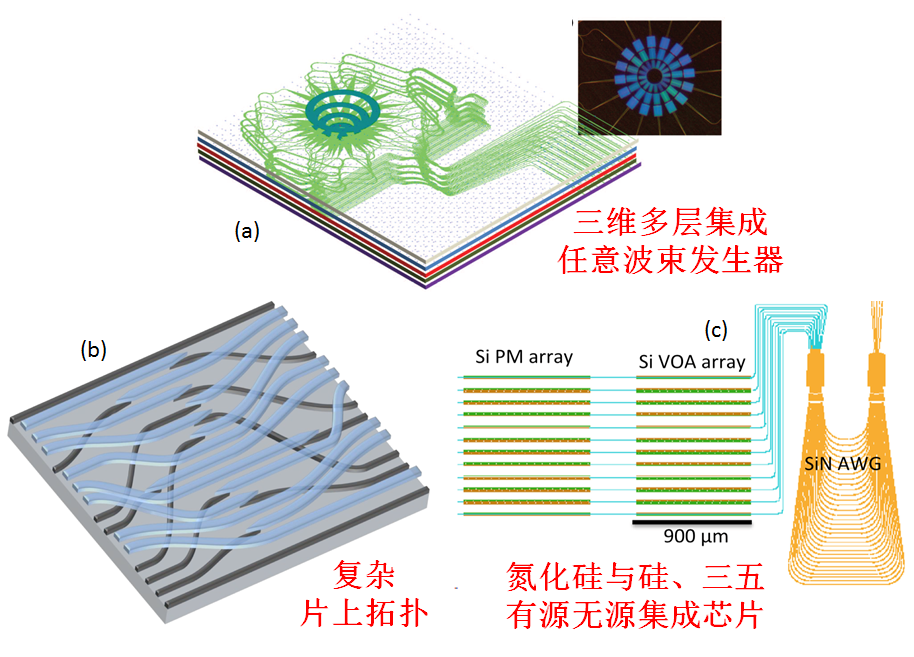
\includegraphics[width=1\textwidth]{Img/4-1.png}
    \caption{典型的氮化硅三维集成的应用前景。(a) 三维多层氮化硅集成的任意波束发射器。(b)复杂的片上拓扑。(c) 氮化硅与硅或三五族半导体材料有源无源混合集成。\cite{Jones2013Ultra,Yoo2016Heterogeneous,Dong2016Silicon}}
    \label{fig:4-1}
\end{figure}
%%%%%%%%%%%%%%%%%%%%%%%%%%%%%%%%%%%%%%%%%%%%%%%%%%%%%%%%%%%%%%%%%%%%%%%%%%%%%%%%%%%%%%%%%%%%%%%%%%%%%%%%%%%%%%%%%%%%%%
如第3章第一节所述,氮化硅作为一种新兴的集成光子材料体系,具有优异的光学特性,还可以进行便捷的化学气相沉积,方便地沉积到不同的材料表面上,实现三维的光子集成。\cite{Xie:15,Geyter2012From}

氮化硅的三维集成,有三类典型的应用领域,如图4.1所示,一种是通过多层氮化硅波导的三维层叠,通过多层三维集成的极高自由度,实现任意波束的片上发射,如图4.1a,加州大学戴维斯分校的S. J. Ben Yoo团队提出的通过五层的氮化硅波导的多层布局,通过环形的氮化硅光栅的相干叠加光束射,可以实现任意波束的发射。\cite{Yoo2016Heterogeneous}

第二种是可以实现复杂的片上拓扑结构,如图4.1b为美国桑迪亚国家实验室的Adam M. Jones等人展示的16×16通道的BANYAN网络,通过传统单层的光子波导很难实现复杂的网络拓扑的连接。而通过,通过氮化硅的三维集成的辅助,则可以方便地解决复杂光网络的连接问题。\cite{Jones2013Ultra}

第三种则是通过氮化硅与成熟、功能完善的硅基光子电路或三五族光子电路的混合集成,通过氮化硅材料的低损耗、高容差特性的优势,结合有源材料的有源器件功能,实现混合集成光子电路的进一步性能突破。 
 
硅材料则作为成熟的集成光子材料体系之一,具有较高的折射率和高集成度的优势。而三五族半导体材料在激光器、光调制器和光探测器等有源集成中也有广泛的应用。由于硅和三五族材料的折射率较高,高折射率的光子器件的性能容易受到器件加工误差的影响,导致串扰增大和性能降低等负面结果。

通过硅、三五族半导体和氮化硅的混合集成,一方面,可以兼有高折射率硅和三五族集成光子芯片的成熟、高集成度和多功能优势;另一方面,结合了氮化硅的低热光系数、低非线性、低折射率、高容差特性的优势,可以制备更高性能的混合集成光子芯片。如美国贝尔实验室的Po dong等人和加州大学圣塔芭芭拉分校的Molly Piels等人,通过氮化硅的阵列波导光栅AWG和硅、磷化铟的三五材料体系混合集成,制备了更低串扰的DWDM光接收模块。\cite{Dong2016Silicon,Bauters2014Low}

综上所述,氮化硅的三维混合集成具有明确有效的应用前景。在氮化硅的混合三维集成中,需要将光从硅、三五族材料中耦合到氮化硅层,需要通过精心设计的层间耦合器来实现波导的层间耦合。

在本章中,主要考虑硅与氮化硅波导的层间耦合。

\section{硅与氮化硅层间耦合器的文献调研}

\begin{figure}[!htbp]
    \centering
    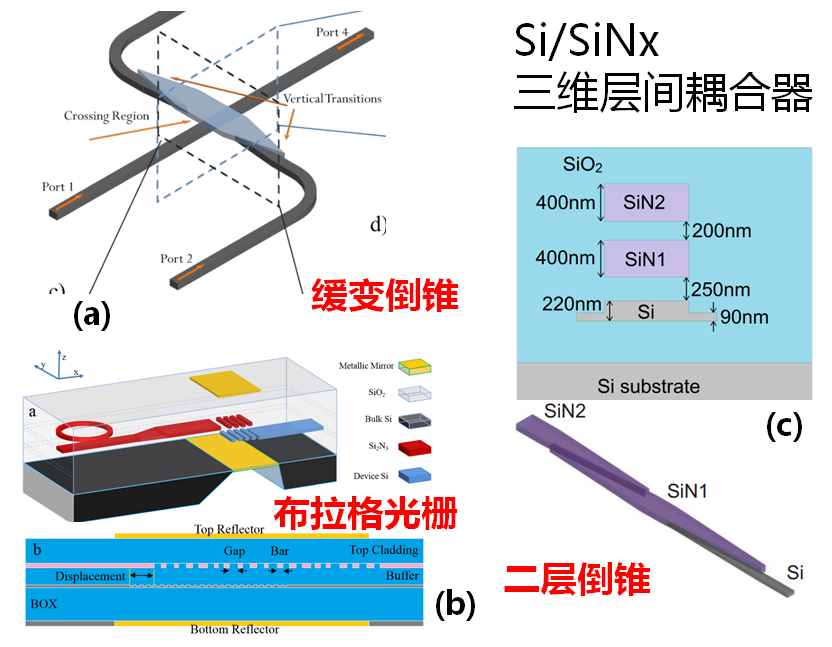
\includegraphics[width=1\textwidth]{Img/4-2.png}
    \caption{已报道的硅-氮化硅层间耦合器的层间耦合方案。(a) 简单有效的缓变倒锥方案。(b) 类似于光栅耦合器的布拉格光栅方案。(c) 通过双层的氮化硅的缓变倒锥层间耦合,实现了双倍的超大层间间隔和可忽略不计的交叉损耗。\cite{Jones2013Ultra,Majid2014High,Sacher:17}}
    \label{fig:4-2}
\end{figure}
%%%%%%%%%%%%%%%%%%%%%%%%%%%%%%%%%%%%%%%%%%%%%%%%%%%%%%%%%%%%%%%%%%%%%%%%%%%%%%%%%%%%%%%%%%%%%%%%%%%%%%%%%%%%%%%%%%%%%%
在高折射率的硅和氮化硅的波导层之间,需要层间耦合器来实现光从硅的波导层耦合到氮化硅波导层。通过文献调研,如图4.2所示,常见的层间耦合器类型有:缓变倒锥、布拉格光栅、二层缓变倒锥等方案。

其中,布拉格光栅的方案原理类似于两个光栅耦合器之间的耦合,如图4.2b所示,美国佐治亚理工学院大学的Majid Sodagar等人做了基于上下金属反射层的布拉格光栅方案,其方案特点为器件紧凑,尺寸约20$\mu$m,氮化硅波导层与硅波导层的层间距离足够大,达到1600nm,因而在层间串扰上可以忽略不计\cite{Majid2014High}。然而,布拉格光栅的方案也存在缺点,布拉格光栅之间的耦合效率较低,需要同时采用上下的金属反射层来增大效率,下金属反射层的制备需要在光栅制备流程之前预先沉积好。而预先沉积下金属反射层的步骤,与传统的CMOS工艺的金属化流程不一致,金属的沉积也会为后续的电子束器件曝光增加不可控的因素,对电子束的邻近效应修正等存在影响等。


\begin{figure}[!htbp]
    \centering
    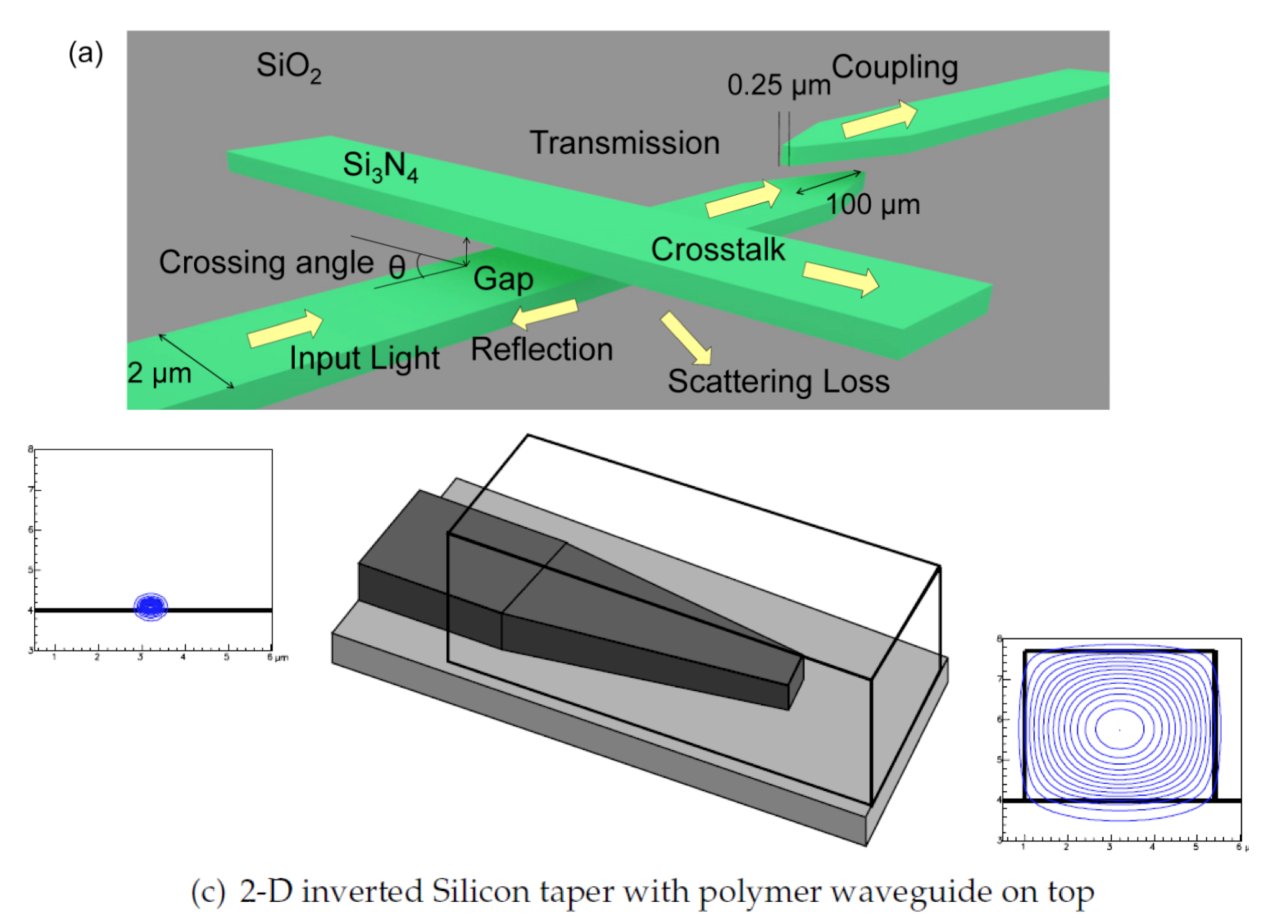
\includegraphics[width=1\textwidth]{Img/4-3.png}
    \caption{倒锥的工作原理示意图,通过倒锥的光限制减弱,光逐步从强限制波导中通过倏逝波的形式弥散到氧化硅的包层中。此时通过另一个相反的缓变倒锥,通过逐步增大波导的模式体积限制,就能耦合到另一层的波导中。\cite{Kuanping2015Low,Dirkgrating}}
    \label{fig:4-3}
\end{figure}
%%%%%%%%%%%%%%%%%%%%%%%%%%%%%%%%%%%%%%%%%%%%%%%%%%%%%%%%%%%%%%%%%%%%%%%%%%%%%%%%%%%%%%%%%%%%%%%%%%%%%%%%%%%%%%%%%%%%%%

目前常用的层间耦合器,大多采用缓变倒锥的方案,如图4.3所示。通过缓变倒锥的结构,使原本局域在硅波导中的强限制光模式,随着硅波导逐渐变窄,模式体积逐渐变大,逐步弥散到二氧化硅的包层中。此时,通过另一个相反方向的氮化硅的缓变倒锥,可以将弥散的倏逝波模式的光从包层重新耦合回氮化硅的波导中,实现光从硅波导层到氮化硅波导层的耦合。\cite{Kuanping2015Low}

如图4.4a所示,硅-氮化硅的缓变倒锥的层间耦合器的主要的指标参数有:硅-氮化硅层间耦合损耗、氮化硅输入交叉损耗、硅输入插入交叉损耗、层间串扰等。

其中硅-氮化硅的层间耦合损耗指光从硅层耦合到氮化硅层的光功率损耗。氮化硅输入交叉损耗指,光在氮化硅波导中传输时,遇到下层相互垂直的交叉硅波导时,产生的插入损耗。硅输入交叉损耗指,光在硅波导中传输时,遇到上层相互垂直的交叉氮化硅波导时,产生的插入损耗。而层间串扰指光在氮化硅波导中传输时,遇到下层相互垂直的交叉的氮化硅波导时,光从上层氮化硅波导耦合到下层硅波导的串扰程度。

\begin{figure}[!htbp]
    \centering
    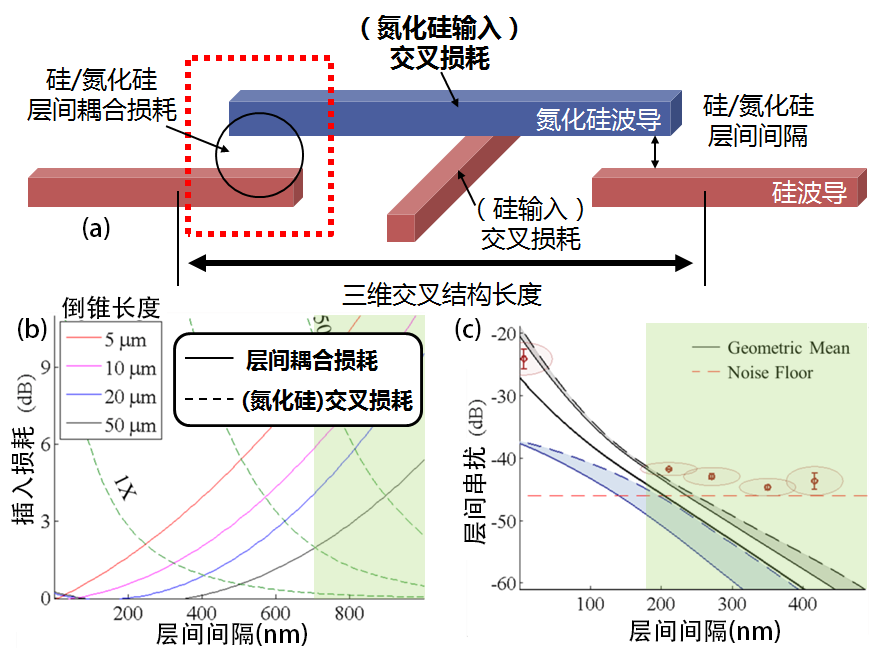
\includegraphics[width=1\textwidth]{Img/4-4.png}
    \caption{(a) 氮化硅-硅的三维层间耦合过程中,主要的器件指标有硅-氮化硅层间耦合损耗、氮化硅输入交叉损耗、硅输入插入交叉损耗、层间串扰。(b) (c)美国桑迪亚国家实验室的Adam M. Jones等人总结的基于倒锥的三维层间耦合光交叉的层间耦合损耗,交叉损耗和交叉层间串扰随着倒锥长度、层间间隔的关系。 \cite{Jones2013Ultra}}
    \label{fig:4-4}
\end{figure}
%%%%%%%%%%%%%%%%%%%%%%%%%%%%%%%%%%%%%%%%%%%%%%%%%%%%%%%%%%%%%%%%%%%%%%%%%%%%%%%%%%%%%%%%%%%%%%%%%%%%%%%%%%%%%%%%%%%%%%

美国桑迪亚国家实验室的Adam M. Jones等人,对倒锥的层间耦合器进行详细的仿真研究,如图4.4b和4.4c展示了,在三维硅-氮化硅的三维混合集成中,在不同的层间间隔以及不同的倒锥长度的情况下,三维交叉的层间耦合损耗、交叉损耗和交叉层间串扰的关系。\cite{Jones2013Ultra}

对于基于缓变倒锥的三维层间耦合器,天然具有很好的层间串扰的特性,只要层间间隔保持200nm以上,便可确保40dB以上的优良的串扰特性。

而层间耦合损耗和交叉损耗需要设计,当倒锥的长度为50$\mu$m时,其总的层间耦合损耗加上氮化硅输入交叉损耗约为1.5dB,总的损耗较大。只有当缓变倒锥的长度增长至大于100$\mu$m时,硅-氮化硅层间距离增大于至少700nm以时,才能使总的损耗降低到可忽略不计的足够低的程度。

对于缓变倒锥的层间耦合器而言,需要足够长的倒锥长度>100$\mu$m的同时,也需要足够大的层间间隔大于700nm才能保证足够高性能的三维层间耦合的集成的需求。

为满足足够大的层间间距,多伦多大学的Wesley D. Sacher等人做了双层倒锥层间耦合器的方案,如图4.2c所示。通过190$\mu$m的器件超长器件长度和双层缓变倒锥形成850nm的较大的层间间隔,取得了-0.15dB三维交叉损耗和和-56dB的层间串扰的极优秀指标。 \cite{Sacher:17}

将调研的已报道的层间耦合器,不同方案的参数指标对比如表4-1所示,可见对于缓变倒锥的方案,其性能指标足够优秀,然而需要相当长的缓变倒锥来实现高性能的耦合,不利于紧凑高集成度的三维集成。需要一种高效而紧凑的硅-氮化硅的层间耦合器,在三维集成芯片中,实现高集成度、高效率的三维光子集成。


\begin{table}[!htbp]
    \caption{图4.2中调研的三种方案的层间耦合器的数据对比}
    \label{tab:5}
    \centering
    \footnotesize% fontsize
    \setlength{\tabcolsep}{4pt}% column separation
    \renewcommand{\arraystretch}{1.2}%row space 
\begin{tabular}{ccccccc}
三维交叉长度             & Si/SiNx间隔 & (氮化硅)交叉损耗 & 层间耦合损耗            & 层间串扰             & 特征                              & 文献       \\ \hline
\textgreater{}50$\mu$m & 410nm     & $\sim$1dB & $\sim$0.5dB       & \textless{}-49dB & {\color[HTML]{FE0000} 缓变倒锥}     & \cite{Majid2014High} \\
190$\mu$m              & 850nm     & 可忽略       & \textless{}0.15dB & \textless{}-56dB & {\color[HTML]{FE0000} 双层倒锥}     & \cite{Jones2013Ultra} \\
$\sim$20$\mu$m         & 1600nm    & 可忽略       & $\sim$0.5dB       & 可忽略              & {\color[HTML]{FE0000} 金属+布拉格光栅} & \cite{Sacher:17} \\
$\sim$20$\mu$m         & 720nm     & 可忽略       & $\sim$0.6dB       & \textless{}-45dB & {\color[HTML]{FE0000} 超材料差拍光栅}  & 本论文     
\end{tabular}
\end{table}
%%%%%%%%%%%%%%%%%%%%%%%%%%%%%%%%%%%%%%%%%%%%%%%%%%%%%%%%%%%%%%%%%%%%%%%%%%%%%%%%%%%%%%%%%%%%%%%%%%%%%%%%%%%%%%%%%%%%%%
%%%%%%%%%%%%%%%%%%%%%%%%%%%%%%%%%%%%%%%%%%%%%%%%%%%%%%%%%%%%%%%%%%%%%%%%%%%%%%%%%%%%%%%%%%%%%%%%%%%%%%%%%%%%%%%%%%%%%%
%%%%%%%%%%%%%%%%%%%%%%%%%%%%%%%%%%%%%%%%%%%%%%%%%%%%%%%%%%%%%%%%%%%%%%%%%%%%%%%%%%%%%%%%%%%%%%%%%%%%%%%%%%%%%%%%%%%%%%

\section{基于拍频的超材料层间耦合器}

\subsection{方案理念}

\begin{figure}[!htbp]
    \centering
    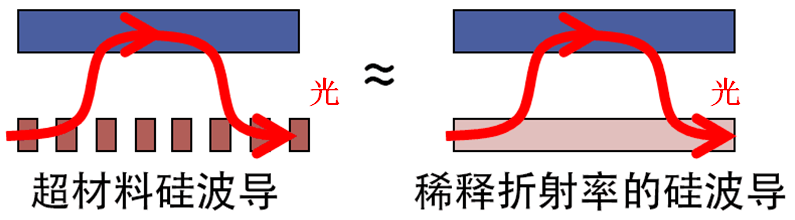
\includegraphics[width=1\textwidth]{Img/4-5.png}
    \caption{基于拍频的超材料层间耦合器的基本原理。通过亚波长光栅的超材料的硅波导,等效为稀释折射率的光波导,实现硅波导和氮化硅波导的折射率匹配。}
    \label{fig:4-5}
\end{figure}
%%%%%%%%%%%%%%%%%%%%%%%%%%%%%%%%%%%%%%%%%%%%%%%%%%%%%%%%%%%%%%%%%%%%%%%%%%%%%%%%%%%%%%%%%%%%%%%%%%%%%%%%%%%%%%%%%%%%%%
如图4.5所示,与传统的缓变倒锥或布拉格光栅的层间耦合器方案不同,通过拍频的超材料层间耦合器,通过在硅波导上刻蚀亚波长的光栅。通过亚波长的光栅,减少硅波导中硅材料的占空比,借此减少硅波导的折射率,实现硅波导折射率稀释。通过匹配稀释硅波导的折射率和氮化硅波导的折射率,可以实现光的差拍光栅耦合,即光在两个相同有效折射率波导中的交替耦合的现象。

差拍光栅的层间耦合方案,相比缓变倒锥,一方面耦合效率接近,光通过差拍直接从硅波导层耦合到氮化硅层,避免了额外的衍射损耗,另一方面,差拍耦合避免了缓变倒锥层间耦合器需要>100$\mu$m足够长的缓变倒锥的缺点,可以实现更为紧凑的层间耦合。

\subsection{二维仿真}

\begin{figure}[!htbp]
    \centering
    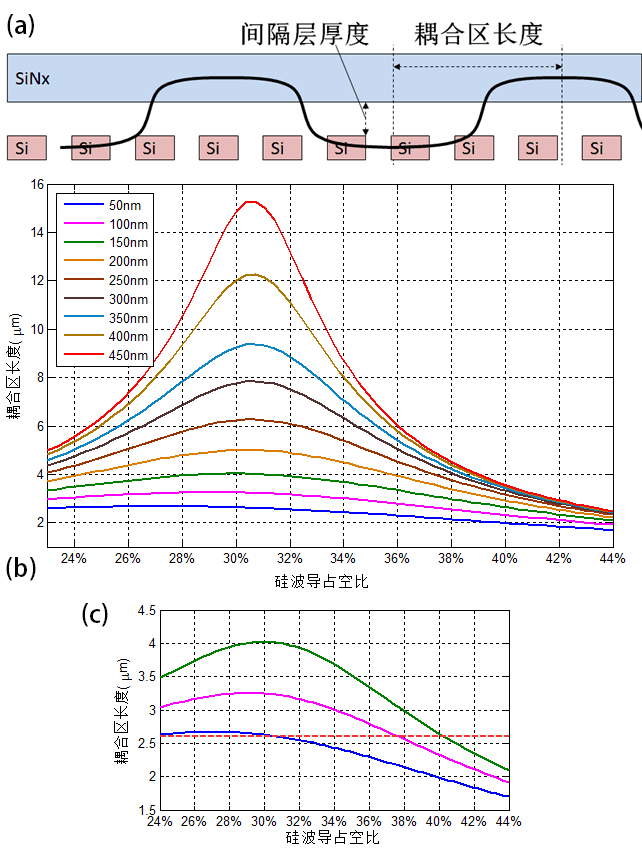
\includegraphics[width=1\textwidth]{Img/4-6.png}
    \caption{拍频层间耦合和层厚度之间的关系。(a) 假想的二维氮化硅平板波导与超材料平板硅波导之间的差拍耦合过程。间隔层厚度和耦合区长度已标注。(b) 不同的硅波导占空情况下,通过超模差拍理论计算的耦合区长度。可见当间隔层厚度越小时,耦合区长度随占空比变化较小。 (c)当间隔层厚度为50nm时,可以在占空比24\%-34\%的范围内保持耦合区长度不变,提供稳定可靠的差拍耦合。}
    \label{fig:4-6}
\end{figure}
%%%%%%%%%%%%%%%%%%%%%%%%%%%%%%%%%%%%%%%%%%%%%%%%%%%%%%%%%%%%%%%%%%%%%%%%%%%%%%%%%%%%%%%%%%%%%%%%%%%%%%%%%%%%%%%%%%%%%%

差拍光栅的方案,先通过二维仿真进行设计,对关键参数进行分析。由于硅的折射率($\sim$3.42)远大于氮化硅的折射率($\sim$2),因此,在二维平板硅波导(Slab waveguide)上刻蚀亚波长的光栅,以稀释硅波导的折射率,匹配氮化硅的平板波导的折射率,实现差拍耦合,如图4.6a所示。波导的四周的空白为二氧化硅包层,折射率为1.4431。

对于硅平板波导到氮化硅平板波导之间的层间耦合,其差拍耦合是通过波导间相互耦合的超模实现,其耦合区长度取决于硅波导的两个基础超模的有效折射率差。

其中,耦合长度可以通过波导间的相互耦合的超模之间传输常数的差值形成拍,其差拍的耦合距离由公式:(详细理论基础参考仿真中关于方向耦合器的tutorial教程)

\begin{equation}
L =   \frac{2\lambda}{n_2-n_1}
\end{equation}

决定,其中,$\lambda$为光模式的真空的波长,而$n_2$是同相位耦合超模式的有效折射率,$n_1$是反相位耦合超模式的有效折射率,一般的有$n_2$>$n_1$。\cite{Foundations,Marcatili1969Dielectric,Trinh1995Integrated}

通过耦合距离公式,分析了不同层间距离、不同的波导占空比的硅波导的情况下,从硅波导到氮化硅波导的耦合区长度,如图4.6b所示。硅平板波导的占空比会随着加工的局限而不可避免的发生偏差,当硅平板波导的占空比发生变化时,耦合长度也相应的发生变化。一般的,如果耦合长度容易随着占空比的偏移而发生较大的变化,则说明层间耦合器的设计对占空比变化敏感,缺乏足够的鲁棒性。

仿真了50$\sim$450nm层间间隔下的耦合情况,可见,当层间间隔越大时,耦合长度随着器件的占空比变化的影响越大,意味着当占空比出现偏差时,耦合的效果就会发生较大的偏差,不利于层间耦合的稳定性;相反,随着层间间隔变小,耦合长度随着器件占空比变化的程度变小。当层间间隔为50nm时,耦合长度可以保持在24\%-34\%的占空比范围内保持约2.6$\mu$m不变。意味着,当层间的间隔为50nm的时候,占空比可以保持±5\%的误差容忍度。而不会因为加工误差而导致性能严重下降,能保证器件的稳定性和加工可行性。

因此,根据二维仿真的结果,将硅波导和氮化硅波导之间的间隔定为50nm,以确保器件有较好的容差特性,便于器件的加工和测试。

在图4.6中,通过二维仿真得到,当氮化硅波导和硅波导的层间距离约50nm时,才能保证足够稳定的层间耦合。而在图4.4中得知,氮化硅波导和硅波导的层间间隔得需要足够大,才能确保足够小的交叉损耗和层间串扰,这是相互矛盾结论。为解决矛盾,采用了双层氮化硅层的方案,如图4.7所示,当光通过超材料的硅波导层,耦合到下层的氮化硅层中;上下两层氮化硅层的厚度一致,有效折射率也一致,因此,光会进一步耦合到上层的氮化硅层,上层氮化硅波导与硅波导的层间间隔较大,避免了交叉损耗。当光绕过下方的硅波导后,再通过相反的过程,逐渐向下耦合,回到超材料的硅波导中。

整个耦合过程为:硅波导→下层氮化硅波导→足够高的上层氮化硅波导→跨过下层的硅波导→下层氮化硅波导→硅波导,实现三维的层间耦合。

\begin{figure}[!htbp]
    \centering
    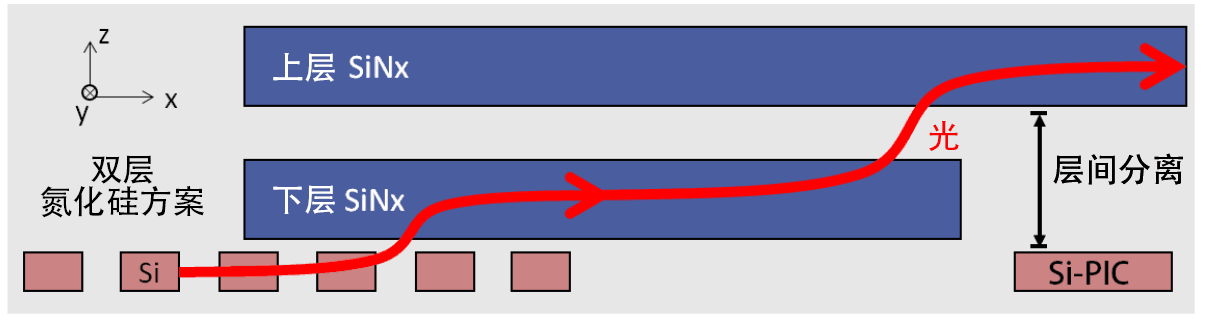
\includegraphics[width=1\textwidth]{Img/4-7.png}
    \caption{双层氮化硅的层间耦合方案,一方面,满足了图4.6中硅-氮化硅层间间隔应该越小越好的要求。另一方面,也满足了图4.4中氮化硅、硅的层间距离要足够大的要求。光从超材料硅波导中耦合到下层氮化硅层,再进一步耦合到上层氮化硅层,使氮化硅和硅层足够的分离,减少交叉损耗和层间串扰。}
    \label{fig:4-7}
\end{figure}
%%%%%%%%%%%%%%%%%%%%%%%%%%%%%%%%%%%%%%%%%%%%%%%%%%%%%%%%%%%%%%%%%%%%%%%%%%%%%%%%%%%%%%%%%%%%%%%%%%%%%%%%%%%%%%%%%%%%%%

\begin{figure}[!htbp]
    \centering
    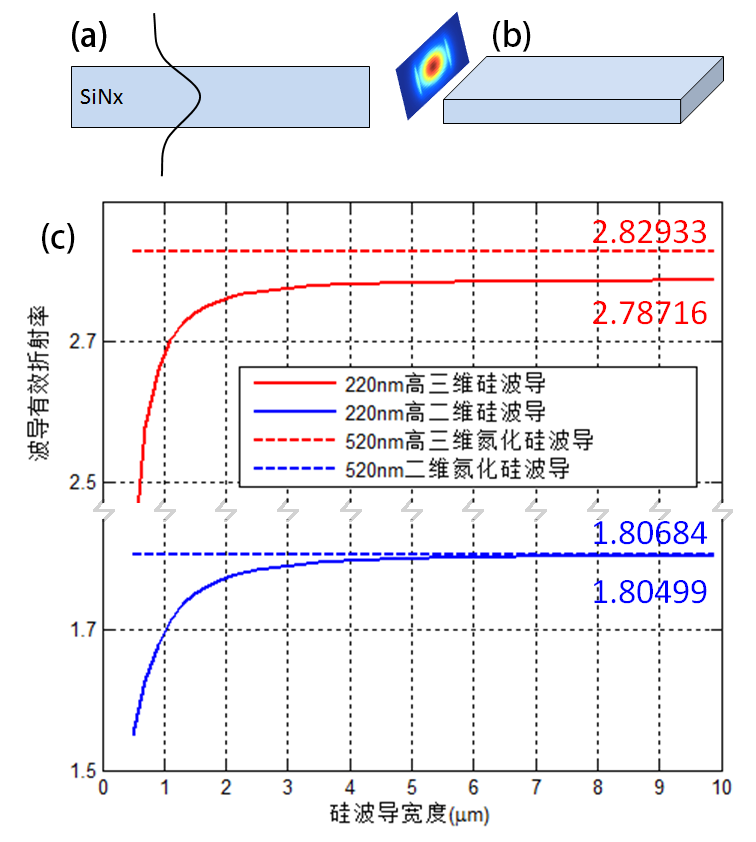
\includegraphics[width=1\textwidth]{Img/4-8.png}
    \caption{(a) 二维无限宽平板光波导的TE模式。(b)三维光波导的TE模式。(c)不同宽度的硅波导和氮化硅波导的有效折射率的情况,当波导宽度大于5$\mu$m时,三维波导的有效折射率接近于二维光波导的有效折射率,可视作准二维的光波导。}
    \label{fig:4-8}
\end{figure}
%%%%%%%%%%%%%%%%%%%%%%%%%%%%%%%%%%%%%%%%%%%%%%%%%%%%%%%%%%%%%%%%%%%%%%%%%%%%%%%%%%%%%%%%%%%%%%%%%%%%%%%%%%%%%%%%%%%%%%

图4.6中的仿真结果是基于二维无限宽的平板硅波导和平板氮化硅波导之间的耦合情况。在实际器件制备中,波导的宽度是有限的。一方面,为了确保器件紧凑高效,波导耦合区的宽度应当尽量小。另一方面,当波导的宽度偏小时,波导传输模式的有效折射率偏小,使得硅波导和氮化硅波导的折射率匹配比较困难。因此,存在一个合理的耦合区波导宽度,使得层间耦合器足够紧凑的同时,确保层间耦合高效鲁棒。

如图4.8所示,分析了不同宽度下的硅波导和氮化硅波导的有效折射率,其中硅波导的高度为220nm,氮化硅波导的高度为520nm。虚线为二维无穷宽的平板波导的有效折射率,可见,对于三维波导而言,当波导的宽度为5$\mu$m后,三维波导的有效折射率趋近于不变或变化缓慢,因此,当宽度为5$\mu$m以上时,波导可以视为准二维的波导,适合作为实际的耦合区的波导宽度。\cite{Luyssaert2005Efficient}

\subsection{三维仿真}

从二维到三维的仿真结构变化,有很大的不同。二维平板波导的占空比调制是通过二维的亚波长光栅实现的,如图4.7所示。其中,要求亚波长光栅的光栅周期足够小,远小于光波长,以避免满足不必要的衍射损耗。当光栅周期远小于波长时,则波导的有效折射率约等于实际波导的有效折射率乘以占空比。

然而,考虑到加工可行性,需要保证足够大的器件特征尺寸,传统的EBL曝光的特征尺寸约为$\sim$100nm \cite{Piggott2017Fabrication},因此本方案中,选择了二维的光栅和一维光栅结合的超材料方案,如图4.9,在实现硅波导与氮化硅波导之间的折射率匹配的情况下,保证有足够大的特征尺寸。

\begin{figure}[!htbp]
    \centering
    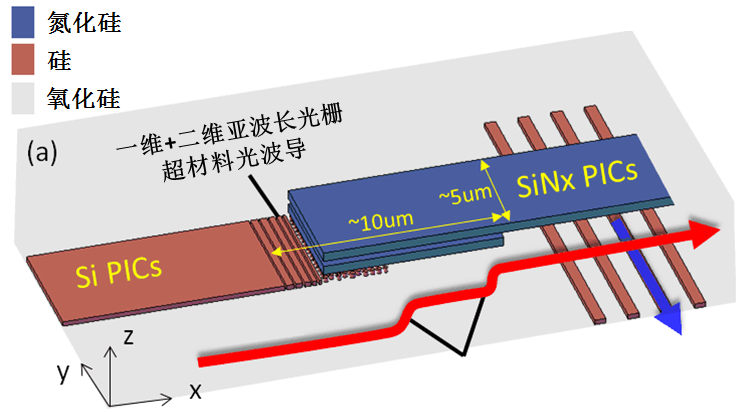
\includegraphics[width=1\textwidth]{Img/4-9.png}
    \caption{一维+二维亚波长光栅双层超材料的层间耦合器方案图,通过一维+二维的亚波长光栅超材料,在实现硅波导和氮化硅波导之间的折射率匹配的情况下,使超材料光波导的最小特征尺寸足够大。}
    \label{fig:4-9}
\end{figure}
%%%%%%%%%%%%%%%%%%%%%%%%%%%%%%%%%%%%%%%%%%%%%%%%%%%%%%%%%%%%%%%%%%%%%%%%%%%%%%%%%%%%%%%%%%%%%%%%%%%%%%%%%%%%%%%%%%%%%%

\begin{figure}[!htbp]
    \centering
    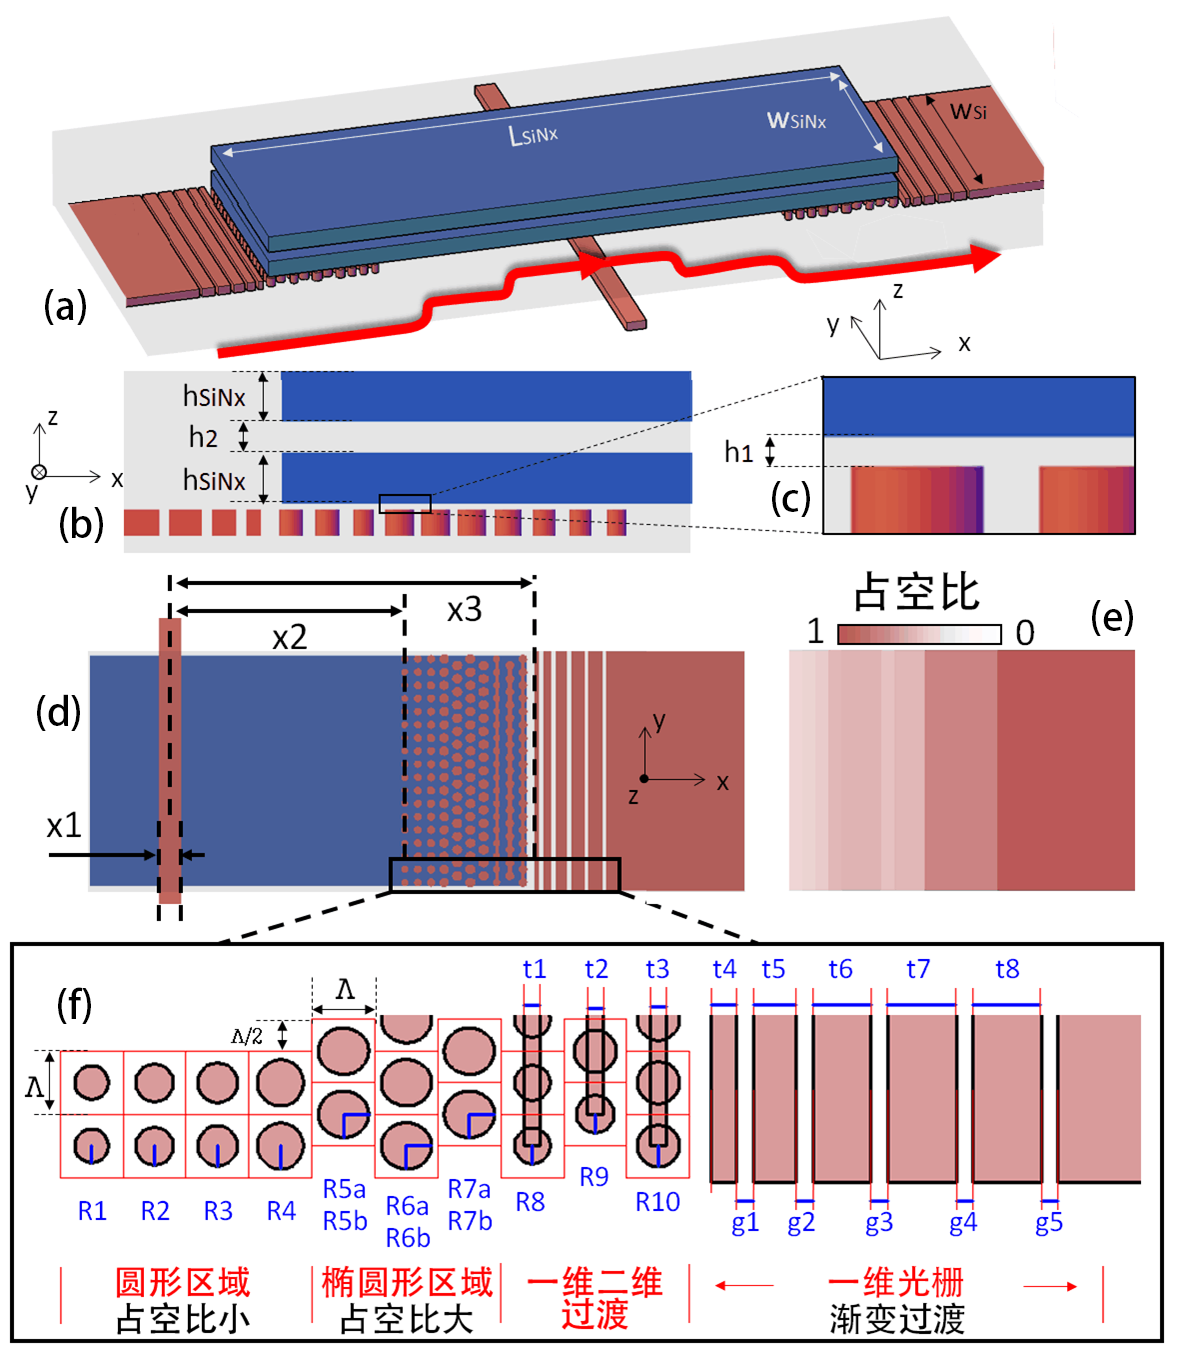
\includegraphics[width=1\textwidth]{Img/4-10.png}
    \caption{超材料层间耦合器的详细结构图,以及与层间耦合器相关的所有结构变量。(a)层间耦合器的整体结构外观,有双层氮化硅的波导层,可以实现光从硅波导→下层氮化硅波导→上层氮化硅波导→下层氮化硅波导→硅波导的耦合过程。(b)层间耦合器的主视图。(c) 硅波导与氮化硅波导之间的极薄的50nm氧化硅间隔层。(d) 层间耦合器的俯视图。(e) 层间耦合器超材料硅波导对应的占空比分布图。(f)层间耦合器的一维+二维超材料光波导的详细结构图,超材料光波导可以划分为用于渐变过渡的一维光栅区域、一维二维的过渡区域、用于较大占空比的椭圆形二维光栅区域、以及较小占空比的圆形二维光栅区域。}
    \label{fig:4-10}
\end{figure}
%%%%%%%%%%%%%%%%%%%%%%%%%%%%%%%%%%%%%%%%%%%%%%%%%%%%%%%%%%%%%%%%%%%%%%%%%%%%%%%%%%%%%%%%%%%%%%%%%%%%%%%%%%%%%%%%%%%%%%

由于采用了二维光栅+一维光栅的超材料的方案,如图4.9所示,通过一维光栅和二维光栅,确保超材料波导的最小特征尺寸足够大。为了便于测试,采用了图4.10a所示的三维交叉,由两个层间耦合器背对背组成。

如图4.10中,列举了所有结构相关的变量。一维+二维的光栅结构复杂,为了兼顾占空比的变化和足够大的特征尺寸,将超材料波导分成了四个部分,分别为:一维光栅、一维二维过渡,椭圆形二维光栅,圆形二维光栅,如图4.10f所示。其中一维光栅用于光波导从普通波导到超材料波导之间的渐变过渡,一维二维光栅用于一维光栅与二维光栅之间的过渡,椭圆形二维光栅用于高占空比的二维光栅,椭圆形可提升特征尺寸,避免二维光栅柱,而圆形二维光栅用于低占空比的二维光栅。\cite{Bock2010Subwavelength}

在器件设计中,涉及的结构变量比较多,有36个变量,如表4-2所示。因此器件的设计过程中需要合理的变量优化算法,采用了遗传算法的方式进行优化。

遗传算法优化的过程是通过Lumerial内置的脚本语言实现的,如图4.11,TE基模从端口1输入硅波导然后不断优化表4-2中的变量,而仿真的目标函数为,优化从1端口输入2端口输出的光功率,最小化插入损耗。

通过遗传算法的优化,对应的结构参数如表4-2所示。其中超材料硅波导的最小特征尺寸限制为80nm以上,可以通过电子束曝光EBL进行制备。


\begin{table}[!htbp]
    \caption{通过遗传算法优化的图4.10中结构变量的具体参数。(单位nm)}
    \label{tab:5}
    \centering
    \footnotesize% fontsize
    \setlength{\tabcolsep}{4pt}% column separation
    \renewcommand{\arraystretch}{1.2}%row space 
\begin{tabular}{ccccccccc}
R1   & R2   & R3  & R4    & R5a & R5b & R6a  & R6b   & R7a   \\ \hline
80   & 90   & 95  & 110   & 120 & 110 & 120  & 110   & 120   \\
R7b  & R8   & R9  & R10   & t1  & t2  & t3   & t4    & t5    \\ \hline
110  & 85   & 100 & 100   & 80  & 80  & 80   & 120   & 200   \\
t6   & t7   & t8  & g1    & g2  & g3  & g4   & g5    & x1    \\ \hline
275  & 325  & 325 & 85    & 85  & 80  & 80   & 80    & 500   \\
x2   & x3   & Λ   & $h_{SiN}$x & h1  & h2  & wSi  & wSiNx & LSiNx \\ \hline
5350 & 8300 & 300 & 420   & 50  & 260 & 5450 & 5250  & 16250
\end{tabular}
\end{table}
%%%%%%%%%%%%%%%%%%%%%%%%%%%%%%%%%%%%%%%%%%%%%%%%%%%%%%%%%%%%%%%%%%%%%%%%%%%%%%%%%%%%%%%%%%%%%%%%%%%%%%%%%%%%%%%%%%%%%%
%%%%%%%%%%%%%%%%%%%%%%%%%%%%%%%%%%%%%%%%%%%%%%%%%%%%%%%%%%%%%%%%%%%%%%%%%%%%%%%%%%%%%%%%%%%%%%%%%%%%%%%%%%%%%%%%%%%%%%
%%%%%%%%%%%%%%%%%%%%%%%%%%%%%%%%%%%%%%%%%%%%%%%%%%%%%%%%%%%%%%%%%%%%%%%%%%%%%%%%%%%%%%%%%%%%%%%%%%%%%%%%%%%%%%%%%%%%%%

\begin{figure}[!htbp]
    \centering
    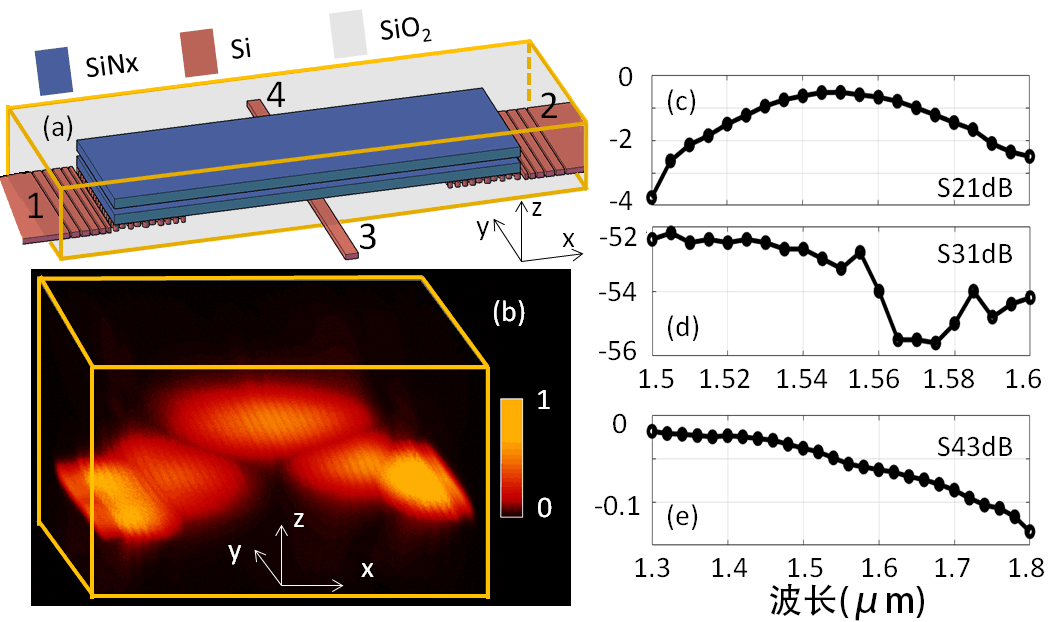
\includegraphics[width=1\textwidth]{Img/4-11.png}
    \caption{(a) 层间耦合器的三维交叉对应的四个端口1,2,3,4。(b) 通过Lumerical 3D-FDTD在1端口输入TE模式的光后,得到层间耦合器电场分布,可以看到光从硅波导逐步向上耦合至上层的氮化硅波导中,越过下端的硅波导后,逐步向下耦合,从端口2的硅波导中输出,与设计的光路径一致。(c) 通过3D-FDTD仿真得到的S21dB插入损耗,中心波长1550nm处损耗仅为0.52dB。(d)仿真得到的S31dB三维交叉层间串扰,整体的串扰水平在-52dB以下。(e) 仿真得到的S43dB硅输入交叉损耗,通信波段交叉损耗的整体在-0.1dB以内。}
    \label{fig:4-11}
\end{figure}
%%%%%%%%%%%%%%%%%%%%%%%%%%%%%%%%%%%%%%%%%%%%%%%%%%%%%%%%%%%%%%%%%%%%%%%%%%%%%%%%%%%%%%%%%%%%%%%%%%%%%%%%%%%%%%%%%%%%%%

在完成了上述的遗传算法变量优化之后,通过Lumerical 3D-FDTD对器件进行了详细的仿真,主要仿真了三维层间耦合过程中的电磁场分布、插入损耗、层间串扰和波长响应等情况,如图4.11所示。.

如图4.11b所示,通过在图4.11a的1端口,输入基础TE模式,可以看到,仿真得到的电场分布符合设计的预期,TE模的光源从端口1输入后,耦合到下层的氮化硅层后又逐步攀登到上层的氮化硅层,越过下方的硅波导后,又向下耦合回超材料硅波导。通过电场图的分布,可以直观地说明双层氮化硅的设计的方案是有效的。

如图4.11c所示,可见,在仿真C波段的中心波长1550nm处,理论的最低插入损耗为-0.52dB,相当于单个层间耦合器的损耗为-0.26dB。而层间串扰如图4.11d,则低于-52dB,层间的串扰相比平面的光交叉要好12dB以上。随着光波的波长发生变化,偏离了中心波长后,插入损耗会逐步增加,而层间串扰则保持在-52dB以下。说明了当波长偏离后,层间耦合的损耗会增加,但不会增加层间串扰,相比单层的光交叉,在实际的应用中具有重要意义。

如图4.11e,对于硅输入的交叉损耗,由于硅波导的折射率$\sim$3.42非常大,完全不受上层的氮化硅波导的影响,其交叉损耗仅有<0.1dB,可以忽略不计。

\begin{figure}[!htbp]
    \centering
    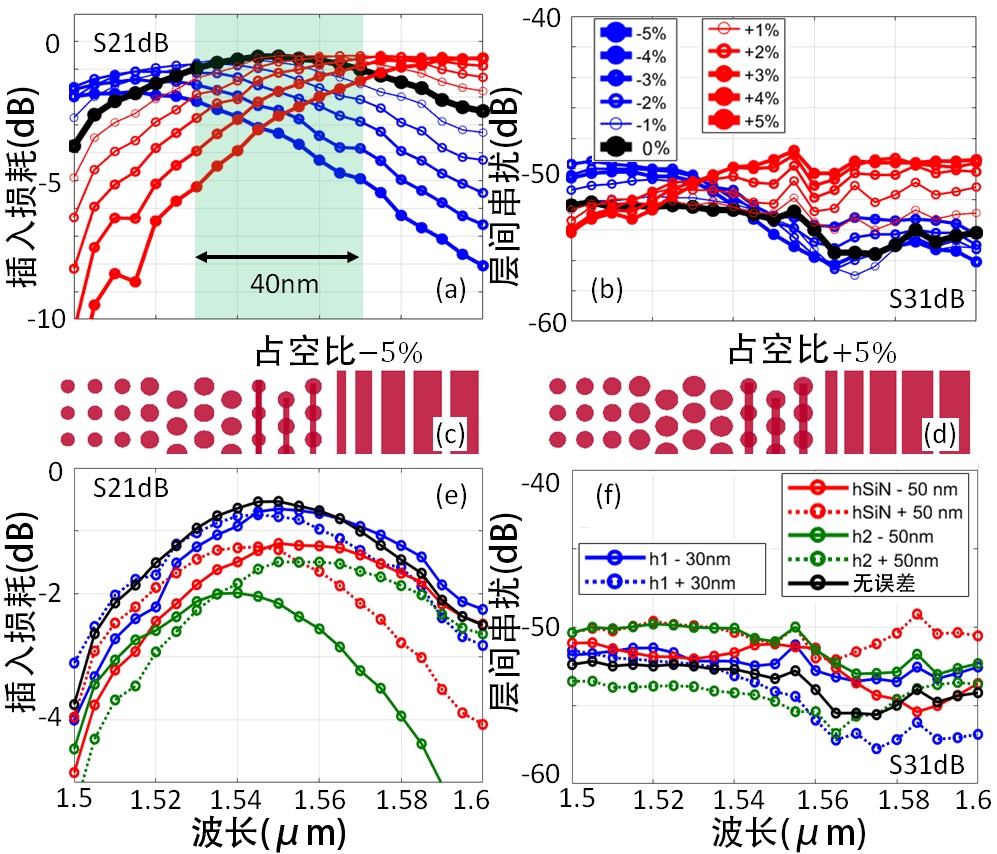
\includegraphics[width=1\textwidth]{Img/4-12.png}
    \caption{层间耦合三维交叉的关键结构的加工容差分析。(a)超材料硅波导的占空比偏移-5\%到+5\%的插入损耗S21dB变化趋势。(b) 超材料硅波导的占空比偏移-5\%到+5\%的三维交叉层间串扰S31dB变化趋势。(c) 超材料硅波导的占空比偏移-5\%时的结构版图示意图。(d) 超材料硅波导的占空比偏移+5\%时的结构版图示意图。(e) 关键的纵向参数,如硅和氮化硅波导间隔h1,氮化硅波导之间间隔h2,氮化硅波导厚度$h_{SiN}$在分别偏差30nm,50nm和50nm时的插入损耗S21dB的变化趋势。(f) 关键的纵向参数在偏差时的三维交叉层间串扰S31dB变化趋势。}
    \label{fig:4-12}
\end{figure}
%%%%%%%%%%%%%%%%%%%%%%%%%%%%%%%%%%%%%%%%%%%%%%%%%%%%%%%%%%%%%%%%%%%%%%%%%%%%%%%%%%%%%%%%%%%%%%%%%%%%%%%%%%%%%%%%%%%%%%

除了FDTD仿真外,还对器件的加工容忍度进行分析,如图4.12所示,其中,分析了部分主要的加工误差项,如超材料硅波波导的加工误差、氮化硅层间之间的厚度、氮化硅厚度的变化误差。

当超材料硅波导的刻蚀发生误差时,比如,占空比整体发生变化,如图 4.12c和4.12d为占空比从-5\%变化到+5\%变化时候的器件版图,且其对应仿真的插入损耗和层间串扰如图4.12a和4.12b所示。可见对于占空比发生变化时,器件的层间串扰几乎没有太大影响,维持在低于-48dB的水平。然而其峰值的耦合效率会发生偏移,当刻蚀的占空比偏差从-5\%到+5\%的时候,其峰值的耦合波长从1.5$\mu$m偏移到1.6$\mu$m处。因此在器件加工的过程中,需要严格的控制电子束光刻、显影以及等离子体刻蚀过程中的占空比变化,使得峰值耦合效率的波长覆盖在所需的C波段范围。\cite{Alexander}

如图4.12e和4.12f所示,在超材料硅波导刻蚀完成之后,上层的氧化硅层厚度和氮化硅波导层的沉积厚度也会随着气相沉积过程的误差而发生偏差,分析了层间厚度h1、h2和氮化硅厚度$h_{SiN}$在±10nm误差下时器件的性能变化,其中在化学气相沉积允许的厚度误差的范围内,器件的损耗变化较小,峰值插入损耗仍能保持在1dB以内,而层间损耗影业能保持在-50dB以下,在实际的气相外延过程中,通过陪片监控,这样的容差结果是可以较好的控制。

\subsection{器件加工与测试}

\begin{figure}[!htbp]
    \centering
    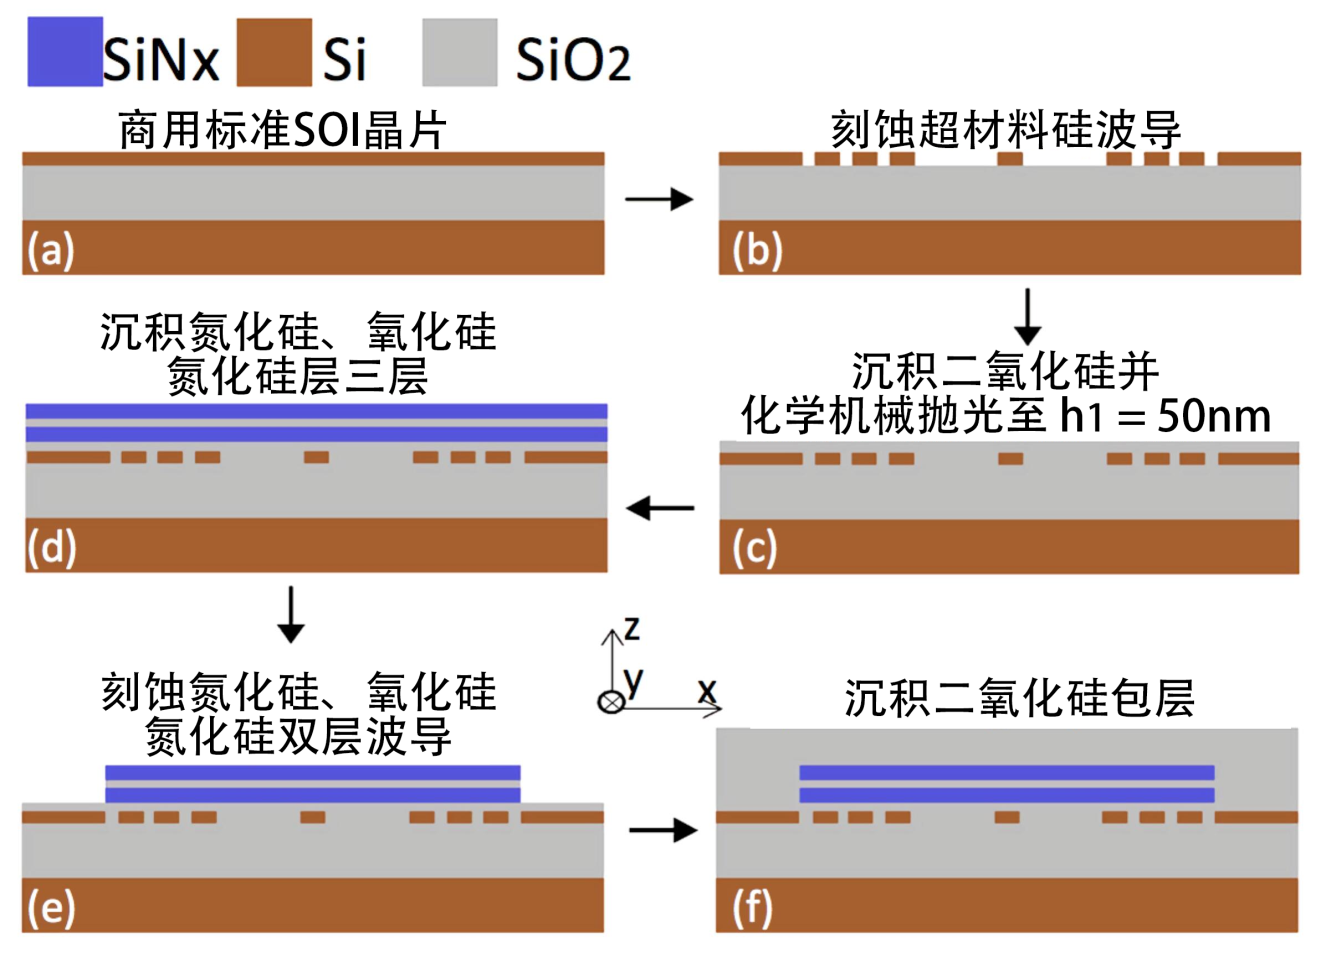
\includegraphics[width=1\textwidth]{Img/4-13.png}
    \caption{器件加工步骤图。(a) 通过商用的220nm的SOI晶片。(2)通过EBL曝光和等离子体刻蚀超材料硅波导。(3)沉积二氧化硅间隔层,并通过CMP进行二氧化硅表面抛光至h1=50nm。(d)依次沉积420nm,250nm,420nm的氮化硅、氧化硅和氮化硅层。(e) 电子束对准曝光并等离子体刻蚀氮化硅、氧化硅、氮化硅双层波导。(f) 在刻蚀完的氮化硅波导上沉积二氧化硅包层,保护波导结构。}
    \label{fig:4-13}
\end{figure}
%%%%%%%%%%%%%%%%%%%%%%%%%%%%%%%%%%%%%%%%%%%%%%%%%%%%%%%%%%%%%%%%%%%%%%%%%%%%%%%%%%%%%%%%%%%%%%%%%%%%%%%%%%%%%%%%%%%%%%

通过电子束曝光,对器件进行加工,如图4.13所示,

(a),首先采用了商用的SOI晶片,需要预先通过lift-off制作金属的对准标记,以便对准曝光时作为参照。

(b),通过电子束曝光ZEP胶,显影并ICP刻蚀,制备超材料硅波导,接着,去除残余的光刻胶。

(c),超材料光波导上沉积足够厚度1$\mu$m的氮化硅,然后通过化学机械抛光(详细的CMP过程及其参数见附录)。通过filmware薄膜测量系统,控制薄膜的厚度,将h1层的厚度抛光至50nm。 

(d),在抛光平滑的样品表面沉积420nm,250nm,420nm的氮化硅、氧化硅和氮化硅层。

(e),通过电子束对准曝光AZ负胶,反应离子束刻蚀RIE,分别刻蚀氮化硅、氧化硅、氮化硅层、形成三层的波导结构,并去除残余光刻胶。

(f),再刻蚀完三层结构的芯片上,生长氧化硅的包层,保护加工好的器件。

\begin{figure}[!htbp]
    \centering
    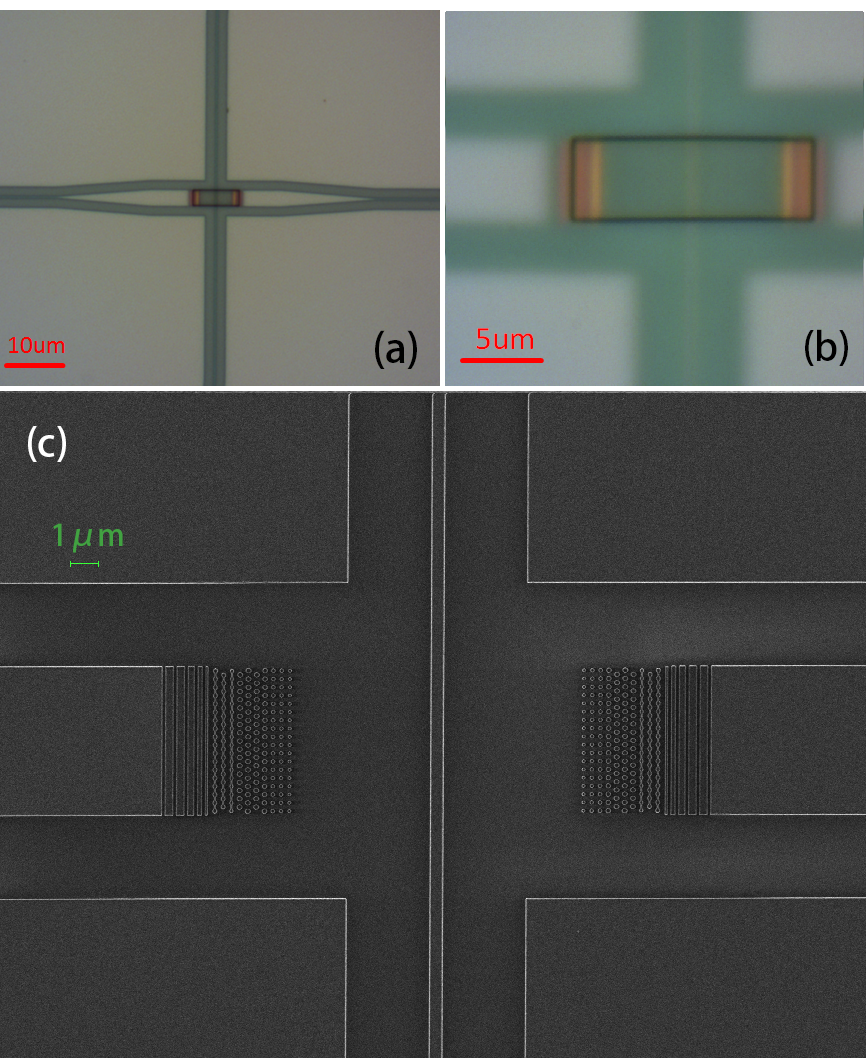
\includegraphics[width=1\textwidth]{Img/4-14.png}
    \caption{(a)制备后的三维交叉层间耦合器在光学显微镜下的结果图。(b) 超材料硅波导上的氮化硅波导层。(c) 制备后的超材料硅波导在电子显微镜下的结果图。}
    \label{fig:4-14}
\end{figure}
%%%%%%%%%%%%%%%%%%%%%%%%%%%%%%%%%%%%%%%%%%%%%%%%%%%%%%%%%%%%%%%%%%%%%%%%%%%%%%%%%%%%%%%%%%%%%%%%%%%%%%%%%%%%%%%%%%%%%%

图4.14为加工后的层间耦合器在光学显微镜下的器件结构图。图4.14a和 图4.14b可以看超材料硅波导上,由于折射率的调控而产生人工色彩的现象。图4.14c是电子显微镜下的超材料硅波导器件的结构,其刻蚀后硅波导的占空比与设计的版图相近。

\begin{figure}[!htbp]
    \centering
    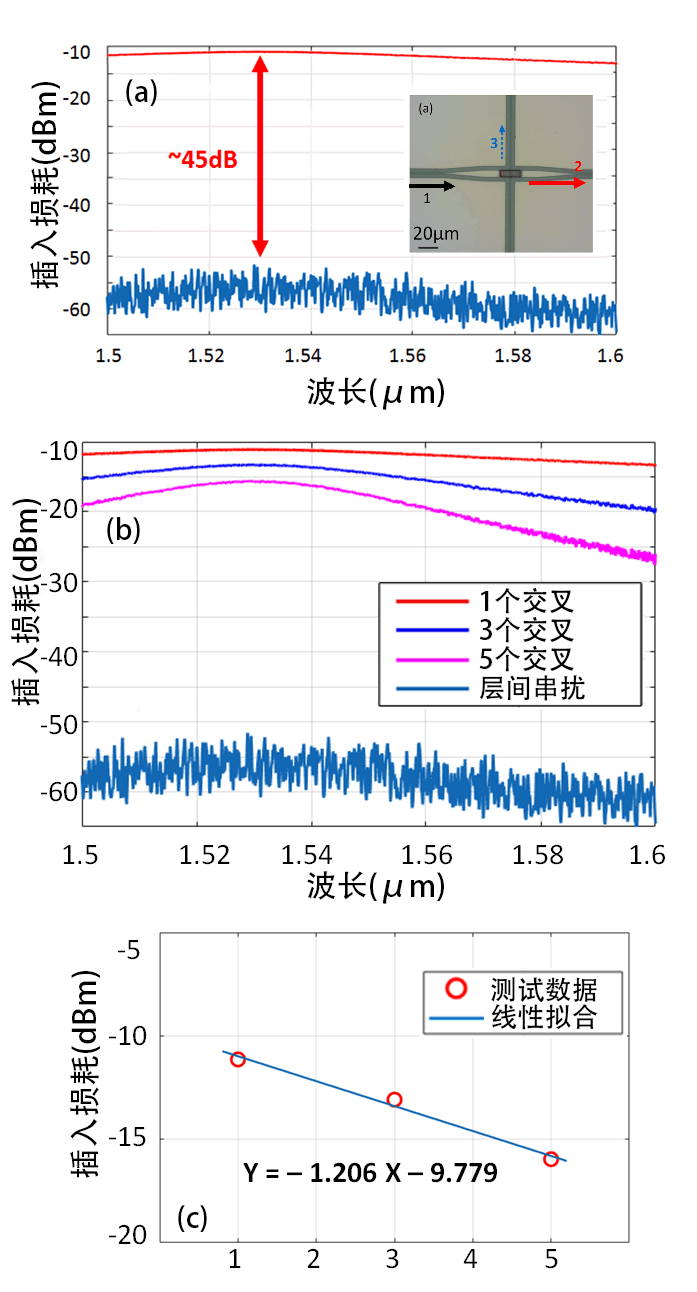
\includegraphics[width=0.8\textwidth]{Img/4-15.png}
    \caption{测试结果图。(a)通过对比S21dB和S31dB的测试数据,可得三维层间交叉的层间串扰大于-45dB。(b) 通过器件测试得到1、3、5个三维层间交叉器件的光纤到光纤投射谱。(c)通过线性拟合不同个数的三维交叉的功率,得到的单个交叉的损耗为-1.206dB。}
    \label{fig:4-15}
\end{figure}
%%%%%%%%%%%%%%%%%%%%%%%%%%%%%%%%%%%%%%%%%%%%%%%%%%%%%%%%%%%%%%%%%%%%%%%%%%%%%%%%%%%%%%%%%%%%%%%%%%%%%%%%%%%%%%%%%%%%%%

对加工后的层间耦合件进行了测试,主要采用了间接测试的方式,通过分析对比不同级联个数的器件的插入损耗和层间串扰,来评估器件的特性。

 
器件的测试设备与3.4章大致相同,采用的是8164B的激光器进行光链路损耗测试。采用了双端锥形光纤耦合,结合偏振控制器来激发光波导中的TE基础模式,使测试得到的光功率最大。当光功率最大时,则说明光波导中的模式以TE模式为主。

在测试过程中,通过控制单一变量方法,测试了单个三维交叉、三个三维交叉、五个三维交叉等不同交叉个数的情况下的链路透射谱,以及层间串扰的透射谱,并通过线性拟合和对比,可以精确的得到单个器件的插入损耗和层间串扰。

 
测试得到的单个三维交叉、三个三维交叉、五个三维交叉的透射谱如图4.15所示,测试的透射谱中包含了光纤—波导的耦合损耗,光纤跳线插入损耗,偏振控制器插入损耗等。
如图4.15a,通过端口1的波导输入TE模式的光,通过对比2端口和3端口出射光功率的功率差,可以得到器件的层间创扰约为45dB。

如图4.15b和4.15c,对比不同三维交叉个数的透射谱,由于最低插入损耗的峰值波长在1531nm左右,通过提取1531nm处的插入损耗并线性拟合,可以得到单个三维交叉的损耗约为-1.206dB@1531nm。

\section{小结}

在本章中,我们提出、设计、加工、测试了一种紧凑的10×5$\mu$m$^2$的超材料硅与氮化硅波导的层间耦合器,并创新性的采用了双层氮化硅的波导,在实现了稳定的硅-氮化硅层间耦合的情况下,又保证了足够大的层间间距。相比于传统的倒锥层间耦合器,具有紧凑高效率的特点。我们通过三维交叉结构来测试层间耦合器的性能,通过器件测试得到的三维交叉的插入损耗为-1.206dB@1531nm,即单个层间耦合器的损耗约为-0.6dB,且1dB带宽覆盖了所需要的1530-1570nm波段,通过这紧凑的三维层间耦合器,可以较好的满足密集的三维层间耦合应用的需求。\cite{Xu:19}
